\documentclass[../thesis.tex]{subfiles}
\begin{document}
\chapter{Future Research}

\subsection{Summary of This Work}

This thesis has sought to increase the understanding of OLED device behavior from a fundamental physics standpoint.
This has focused on three main topics, being device dynamics modeling, device lifetime decoupling, and attempting to develop molecular design rules.
Rather than focusing on offering peak device performance, these studies have tried to present techniques for better understanding device behavior, allowing more informed optimization of peak devices.
These research areas reflect the state of the field and limitations of further commercialization.
The unique capabilities this previous research has developed within our group has enabled several potential future research directions.

In Chapter \ref{sec:unified} an existing model for exciton dynamics within an OLED was extended to include polaron dynamics, allowing the fitting of transient and steady-state dynamics using the same fitting constants.
This additionally allowed for the extraction of the charge balance factor, and quantification of these dynamics as the exciton formation efficiency.
While attempts to utilize this improved dynamics model to quantify material differences have not been done extensively, the better understanding of polaron dynamics and exciton formation has triggered a different mindset for dissecting device behavior and analyzing results in both the steady-state, and lifetime.

In Chapters \ref{sec:integrated_lifetime} and \ref{sec:decoupling_applications} an approach for decoupling lifetime into component efficiencies was developed.  
Taking the understanding of device operation developed in Chapter \ref{sec:unified}, intrinsic device degradation can be thought of as a combination of \pl and \oc loss over time.
This has proven to be a very useful tool for understanding lifetime behavior.  
Chapter \ref{sec:decoupling_applications} talks about three studies where this technique has provided valuable information, specifically in regard to the recombination zone width and position dependence.
One limitation of this technique is that the degradation products are not known, only how it is affecting the device performance.
This can make it difficult to attribute degradation problems to an individual molecule directly.
However, this is still more information than just looking at the EL decay, so provides more information.

An understanding of design rules for OLED molecules was also considered.
In Chapter \ref{sec:hoye}, development of blue fluorescent emitters was considered along with device performance, while Chapter \ref{sec:hosts} took an alternative approach and investigated host material performance in device and optical degradation.
In Chapter \ref{sec:hoye}, devices were able to be fabricated with promising efficiency, but lifetimes were extremely unstable.
Investigation of the mechanism for this degradation were not investigated at the time.
Chapter \ref{sec:hosts} investigated EL lifetimes as well as the photostability to get a more fundamental look at degradation and try to attribute aspects of the EL lifetime to individual molecules.

In this chapter, potential future projects are discussed, mostly revolving around lifetime.
Thermally Activated Delayed Fluorescence (TADF) molecules are a recent hot topic in OLEDs, and are a prime candidate for lifetime studies, and could benefit from investigation with our decoupling technique.
During the lifetime decoupling of a device, accuracy of the measurement of \pl relies on a constant \oc.
It is therefore important that the RZ of the device does not move during degradation, a claim that is largely uninvestigated, and could use further investigation.
%Finally, using similar methods to the decoupling technique of Chapter \ref{sec:integrated_lifetime}, single carrier and optical degradation can help to further isolate degradation pathways.
All of these topics are discussed in detail in this chapter.

\subsection{TADF Lifetime Decoupling}

\begin{wrapfigure}{r}{.5\textwidth}
\centering
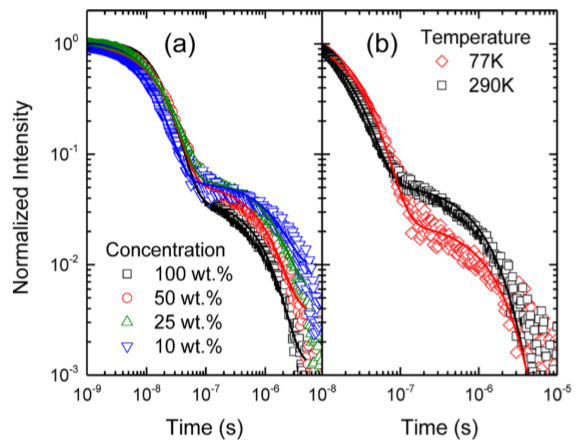
\includegraphics[width=.5\textwidth]{future/pl_lifetime}
\caption{Transient PL lifetime of 4CzIPN, a TADF emitter.  A short and long lifetime component are observed with lifetimes $\approx 1\ ns$ and $\approx 1\ \mu s$.  Figure reproduced from \textcite{Menke2016}.}
\label{fig:future_pl_lifetime}
\end{wrapfigure}

Thermally Activated Delayed Fluorescence (TADF) is a promising OLED technology that has yet to see large commercial usage.\supercite{Endo2009,Zhang2012b,Uoyama2012,Zhang2012c,Li2013}
In TADF molecules, the energy difference between the singlet and triplet is similar to the thermal energy at room temperature.  
This allows triplet molecules to transfer back into the emissive singlet, providing an alternative method to achieve $\chi=1$ without phosphorescence and the use of rare earth heavy metals.
In addition to the potentially cheaper synthesis, TADF materials have been shown to improve exciton transport,\supercite{Menke2016} as well as a reduced efficiency roll-off\supercite{Inoue2016,Wang2015} and long lifetime.\supercite{Cho2014,Mehes2014}
Some believe that TADF will replace Metal Ligand Charge Transfer (MLCT) molecules in commercial devices.\supercite{Reineke2014a}

With a large amount if interest, it is important to investigate device lifetimes.
Promising initial results have shown operational $t_{90}>200$ hours for a green emitter at 1000 cd/m$^2$.\supercite{Cho2014}
This is not sufficient for commercial devices, but needs further development and optimization.
With TADF only being realized in the last half decade, this technology does not share the same long history of development of fluorescent and phosphorescent emitters.\supercite{Tang1987,Tang1989a,Baldo1998a,OBrien1999a,Baldo2000}
Therefore, it does not share in the long history of brute-force optimization and understanding of limiting processes for lifetime through experience.
Using the lifetime decoupling technique described in Chapter \ref{sec:integrated_lifetime} could help to rapidly improved the understanding of TADF device operation.


One of the key parameters of a TADF emitter is the reverse intersystem crossing rate, $k_{RISC}$.\supercite{Uoyama2012,Zhang2012c,Menke2016,Yersin2014,Jankus2014}
The population rate equations for singlets and triplets in a TADF system can be described as \supercite{Menke2016}

\begin{eqnarray}
\frac{dn_S}{dt} &= -n_S(k_{R,S}+k_{NR,S}+k_{ISC})+n_{T}k_{RISC}+G \label{eqn:tadf_ns} \\
\frac{dn_T}{dt} &= -n_T(k_{NR,T}+k_{RISC})+n_Sk_{ISC} \label{eqn:tadf_nt}
\end{eqnarray}

where $n_S$ and $n_T$ are the singlet and triplet densities, respectively, $k_{R,S}$ and $k_{NR,S}$ are the radiative and non-radiative singlet rates, $k_{NR,T}$ is the non-radiative triplet rate, $k_{ISC}$ is the intersystem crossing rate, and $G$ is the singlet generation rate.
In this equation, excitons are freely allowed to transfer between the two states via $k_{ISC}$ and $k_{RISC}$, but to observe significant delayed phosphorescence, $k_{RISC}$ must be faster than $k_{NR,T}$ and $k_{ISC}$ must be rapid.
The transient photoluminescence of such a system is shown in Figure \ref{fig:future_pl_lifetime}.
Here, a prompt decay is seen on the order of nanoseconds corresponding to rapid decay of the generated singlet population via $k_{R,S}$.
After the prompt component, the remaining excitons undergo ISC and are then limited by $k_{RISC}$, determining the rate of the delayed fluorescence component.

The efficiencies of prompt and delayed fluorescence can be written as

\begin{eqnarray}
\eta_{PL,D} &= \sum_{k=1}^\infty (\Phi_{ISC}\Phi_{RISC})^k \eta_{PL,P} \\
\eta_{PL,P} &= \frac{k_{R,S}}{k_{R,S}+k_{NR,S}+k_{ISC}}
\end{eqnarray}

where $\Phi_{ISC}$ and $\Phi_{RISC}$ are the efficiencies of ISC and RISC in Equations \ref{eqn:tadf_ns} and \ref{eqn:tadf_nt}, respectively.

During lifetime, it is not known what happens to PL degradation.
It is possible that non-radiative rates change, as is the case for phosphorescent emitters, but is also possible that a change in $k_{RISC}$ could occur.
In phosphorescent emitters, $k_{NR}$ is highly influenced by degradation in the surrounding environment.\supercite{Bangsund2018a,Bangsund2018,Hershey2017}
However, a change in $k_{RISC}$ would likely indicate a change in the molecular state of the emitter, or its configuration.
These may have different implications on how to resolve the problem.

To measure $k_{RISC}$ and $k_{NR}$, the transient PL would need to be measured.
This has been done in Chapter \ref{sec:integrated_lifetime} before and after degradation for phosphorescent emitters, trying to separate absorption losses from changes in $k_{NR}$.
This same technique of measuring transients on degraded and undegraded devices could be used as an initial probe to see if any change in $k_{RISC}$ is observed.
If there is a change, transient PL should be incorporated into the degradation setup.
This could replace the steady-state PL measurement, as the steady-state PL information can be extracted from the transient.  
The transient PL integration would require a pulsed laser source into the box, as well as integration of a fast photodiode and oscilloscope.  
This could be limited by equipment, as all of these components are costly.
Alternatively, an approach where multiple degradation points are investigated on different devices could be conducted.
However, this technique utilizing different devices has been previously shown to show a large degree of sensitivity to optical alignment and device-to-device degradation.
This could result in data with too much scatter to resolve the changes in rate constants.

Overall, probing TADF using a decoupled lifetime technique could result in rapid development of understanding of the degradation mechanisms.
This could be of significant interest if a better understanding of $k_{RISC}$ loss over time is developed.
Such information would enable better device optimization, and may inform design rules for better molecular stability of TADF materials.


\subsection{Recombination Zone Movement During Lifetime}

During device operation, modeling attempts and most device understanding of degradation relies on a fixed recombination zone profile.\supercite{Ingram2017,Scholz2015,Giebink2009a,Giebink2008a}
This is a simplifying assumption and results from our own research group on decoupled device degradation suggest that with charge balance degrading, it is unlikely that the RZ is entirely unchanged.\supercite{Bangsund2018,Hershey2017,Bangsund2018a}
A changing recombination zone during degradation would result in a change in the out-coupling efficiency, \oc, as a function of time.  
In simple EL degradation, this could result in a misattribuation of degradation to physical degradation, which may just be an optical effect.
During a decoupled lifetime measurement, a move in the RZ would change the degree of overlap between the EL RZ and the PL absorption, as discussed in \textcite{Bangsund2018}.
Additionally, a change in RZ could result in a change in degradation mechanisms as a function of time, a prospect which is too daunting to have been attempted to explain in previous literature.
To address these issues, it would be informative to track changes in the RZ during degradation.

Chapter \ref{sec:rz_measurement} discussed measurement of the recombination zone in the steady-state undegraded case using a red sensitizer molecule.
This technique used an out-coupling corrected relative peak intensity for a locally sensitized red emitter to indicate RZ presence.
In a series of devices, the RZ can be mapped as a function of position of the red sensitizer.\supercite{Bangsund2018,Hershey2017}
One method of tracking the recombination zone during degradation is to use this same technique as a function of time.
This would require spectral collection as a function of time, rather than the power measurement that is currently employed.  
However, some groups already collect spectral data during lifetime.\supercite{Zhang2017a,Yu2017,Zhang2016b}
In fact, red sensitizers have already been used in lifetime devices for tracking exciton confinement to the emissive layer.\supercite{Coburn2017}

Despite some precedent of similar techniques, great care has to be taken to ensure accuracy of this technique.
First of all, degradation of the red sensitizer must be able to be controlled and isolated.
Ideally, there would be no quenching of the red sensitizer, but it is likely that states that are able to quench the emission of \irppy would be able to quench the sensitizer state.
This makes it extremely difficult to separate movements of the RZ from degradation of the sensitizer.
To control for this, one might create devices featuring extremely narrow and confined RZs where the RZ is not able to move, such as a locally doped SEML device.
This would create a reference for how quickly the sensitizer degrades without allowing movement of the RZ.
An additional problem is in assuring that the sensitizer is not influencing the lifetime it is probing.
Since the red sensitizer is energetically nested within the emitter and host materials, it serves as a deep trap state, which are known to influence device performance.
To counteract this, a low doping concentration would have to be used, and comparison to an undoped control would have to show no changes in the lifetime.
While the testing of this concern is simple, developing a doping scheme that satisfies this condition could be challenging.

If these conditions are met, a significant improvement in degradation mechanics could be enabled.
In our recent study, \textcite{Bangsund2018a}, competing mechanisms of bulk exciton density induced degradation and interfacial degradation were found to be influential.
This was able to be optimized in devices that moved the RZ away from the interface of the HTL.
In a system such as this, degradation could easily be a function of both mechanisms, the ratio of which may depend on the RZ position during degradation.
To be effectively modeled and understood, the RZ must be known throughout the degradation.
In addition to the understanding of particular device systems, this technique would offer great insight in understanding the nature of \ef degradation.
In our previous studies,\supercite{Bangsund2018,Bangsund2018a,Hershey2017} degradation has been decoupled into a \pl and \ef components.
However, exciton formation losses are not further understood in regards to which carrier is suffering a reduction, or where non-radiative recombination centers are forming.
This technique would offer a further handle on understanding this behavior and what is happening to charges as fewer excitons are formed.






\ifcsdef{mainfile}{}{\printbibliography}
\end{document}
